
% The issue addressed in this work is to find an appropriate method to model buoyancy-driven droplets suspensions and more generally disperse multiphase flow throughout statistical modeling.
This work addresses the issue of modeling buoyancy-driven droplets suspensions, and more generally dispersed multiphase flows, with a multiscale modeling approach. 
% Indeed, due to the multiscale physical phenomenon present in those flows it is rather difficult to model the classical governing equations of fluids mechanics.  

The developments presented in this work can be summarized into nine key points:
\begin{enumerate}
    \item 
    In \ref{chap:daniel1} we present a ``hybrid'' set of equations, consisting of phase-averaged equations for the continuous fluid phase, complemented by an arbitrary number of moment conservation equations for the dispersed phase that include interfacial properties of the droplets.
    Additionally, we study the relation between the particle-averaged and phase-averaged equations. 
    We demonstrate that the dispersed phase-averaged equations can be interpreted as a series expansion of the particle-averaged moment equations. 
    \item In \ref{chap:daniel15} we derive the mass, momentum, and energy averaged equations, using the ``hybrid'' formalism, and discuss the phenomena of energy exchanges in emulsions.
    We also provide an explicit and general formulation for the continuous and bulk-phase effective stresses.
    \item In \ref{chap:deformable} we consider droplets with a spheroidal geometry, and show how to derive equations for the tensors that describe the deformation and rate of deformation of the droplets. 
    This leads to a set of equations that is similar to the classic models that describe the oscillation of the second mode of deformation of a droplet but including the explicit formulation of the forcing term as a function of the local properties of the flow. 
    \item     
    In \ref{chap:daniel2} we propose a generic approach to derive the \textit{single-particle conditional averaged} Navier-Stokes equations. 
    Then, we revisit the derivation of (2.10) of \citet{batchelor1972sedimentation} which relates the ensemble-averaged properties of the continuous phase to \textit{single-particle} conditionally averaged quantities.
    Notably, we show that the assumptions made by \citet{batchelor1972sedimentation} to derive this formula are not sufficient to get the expression given in his paper.
    This explains the convergence issues sometimes encountered when using this relation \citep{batchelor1972sedimentation}. 
    \item In \ref{chap:closure-disperse}, we derive the closure terms present in the ``hybrid'' model for suspensions made of spherical droplets in the dilute and Stokes flow regimes. 
    While many of these were already established \citep[Appendix A]{zhang1997momentum}, we introduced several new closures.
    Specifically: 
    The pseudo-turbulent stress $\avg{\chi_f \textbf{u}_f'\textbf{u}_f'}$ generated by a mean shear flow on the droplets; 
    The pseudo-turbulent kinetic energy transfer resulting from the local work on the surfaces of the droplets; 
    The droplets induced dissipation term, $\avg{\chi_f \bm\sigma_f^0:\grad \textbf{u}_f^0}$; 
    The term representing the averaged viscous dissipation within the droplets. 
    The term representing the averaged kinetic energy within the droplets. 
    \item We propose an analysis of the mean deformation of droplets, and of the effective stress of the suspension, in the presence of mean relative motion between the phases and considering small-but-finite inertial effects. 
    With the reciprocal theorem we show that the \textit{stresslet} term has a contribution proportional to the mean relative velocity squared. 
    We deduce that, because of the \textit{stresslet} term, a uniform relative translation between phases induces the deformation of the droplets and additional stresses in the suspension. 
    The analytical expression of the \textit{stresslet} is then compared to the numerical results and good agreement is obtained. 
    This contribution is also compared to the \textit{Reynolds} stress term. 
    We conclude that both contributions are of the same order of magnitude in the moderately dense regime ($\phi =0.2$). 
    \item In \ref{chap:mono-disperse}, we propose a new drag force model taking into account an arbitrary viscosity ratio, $\lambda$. 
    The model is built on already existing correlations valid at $\lambda\to\infty$ and $\lambda = 0$, and combines the Richardson-Zaki relation, Schiller-Neuman, and Mei drag force coefficients.
    We then show based on the DNS results that it is also valid at intermediate values of $\lambda$.
    The main advantage of this model is its robustness since the Richardson-Zaki relation is valid at very high volume fractions  ($\phi \approx 0.5$), while in the dilute limit the Schiller-Neuman, and Mei drag force coefficients are proven to be accurate up to $Re = 800$. 
    Thus, we provided a robust drag force coefficient that can directly be used in Euler-Euler frameworks for simulations of emulsions at arbitrary $\lambda$.   
    \item In \ref{chap:pseudoturbulence} we derive an analytical formula for the \textit{Reynolds} stress tensor in the low inertia and dilute regime, for an arbitrary viscosity ratio $\lambda$. 
    Then we use the numerical results (see \ref{chap:DNS}) to extend the validity of this model to arbitrary $Re$ and $\phi$. 
    Good agreement is obtained when comparing our model to experimental results of the literature for solid particles and bubbles.  
    \item Finally, in \ref{chap:microstructure,chap:microstructure_kin} we provide a methodology to characterize the microstructure geometry and microstructure kinematics of a buoyant emulsion. 
    The geometry is characterized using the nearest-neighbor distribution, which is evaluated as a function of the dimensionless parameters. 
    % We also developed tools characterizing the 
    We then determine the relaxation time that it takes for the microstructure (characterized by the nearest-neighbor distribution) to reach its stationary equilibrium geometry, and describe the kinematics of interactions between pairs of droplets. 
\end{enumerate}

We would like to end this conclusion by presenting what we believe is the simplest averaged model that describes the momentum of a buoyancy-driven droplets suspensions. 
Assuming that the kinetic energy of the continuous phase follows a quasi-steady-state equilibrium, we may write the averaged momentum conservation of the continuous phase as, 
\begin{align}
    % &\pddt (\phi_f \rho_f)  
    % + \div (
    %     \phi_f \rho_f\textbf{u}_f
    % )
    % = 
    % 0,\\
    % \pddt (\phi_f\rho_f \textbf{u}_f)
    % + \div (\phi_f\rho_f \textbf{u}_f\textbf{u}_f)
    \phi_f\rho_f (\pddt + \textbf{u}_f\cdot \grad)\textbf{u}_f
    = \phi_f 
    \left(\div \bm{\Sigma}_f
    + \rho_f \textbf{g}\right)
    + \div  \bm{\sigma}_f^{\text{eff}}
    - n_p \textbf{f}_p,
    \label{eq:momentum}
\end{align}
with, 
\begin{align}
    n_p \textbf{f}_p  
    &= 
    \underbrace{f(Re,\phi, \lambda) \times \textbf{u}_{fp}}_\text{Drag force}
    \label{eq:draggggg}
    \\
    \label{eq:newtonian}
  \bm\Sigma_f &= - \underbrace{p_f \bm\delta + \mu_f [\grad \textbf{u}_f +  (\grad \textbf{u}_f)^\dagger ]}_\text{Averaged newtonian stress} 
  \\
    \bm{\sigma}^{\text{eff}}_f 
    &= \underbrace{ C_E(Re,\phi,\lambda)  [\grad \textbf{u}_f +  (\grad \textbf{u}_f)^\dagger ] }_\text{``Einstein viscosity''-like contributions}
    \nonumber\\
    &+ 
    \underbrace{
      C_1(\phi,\lambda,Re)\textbf{u}_{fp}\textbf{u}_{fp}
      +  C_2(\phi,\lambda,Re)(\textbf{u}_{fp}\cdot \textbf{u}_{fp})     \bm\delta}_\text{Particle Induced Turbulence and Stresslet contributions}
    \label{eq:stress}
\end{align}
Where \ref{eq:momentum} is complemented by the momentum equation of the dispersed phase and the corresponding mass conservation for both phases. 

% In this case, the dominant contribution of the drag force term is its component proportional to the relative velocity $\textbf{u}_{fp}$. 
A model for the drag force, which is represented by the scalar function $f$, is given in \ref{chap:mono-disperse}. 
The scalar $C_E$ represents the contribution of the \textit{stresslet} term.
It can be interpreted as an additional coefficient for the continuous phase viscosity, as this term is proportional to the mean rate of strain of the continuous phase \eqref{chap:closure-disperse}.
The coefficients $C_1$ and $C_2$ are more complex. 
They represent the contribution of the \textit{stresslet} term (see \ref{chap:closure-disperse}) and also of the Reynolds stress tensor (see \ref{chap:pseudoturbulence}). 



As seen in \ref{chap:closure-disperse} (see also \ref{ap:momentum_formulation}) the formulation given by \ref{eq:draggggg,eq:stress} does not include all the closure terms. 
Indeed, $\textbf{f}_p$ and $\bm\sigma_f^\text{eff}$ should also take into account the effect of the relative acceleration between phases (added mass effects), the effects of non-homogeneity, etc.
More generally these terms should include all the other physical contributions that were not taken into account in the steady-state, mono-disperse, and homogeneous flow situation. 
Nevertheless, we state that \ref{eq:draggggg,eq:stress} although not complete, constitute the simplest approach to model buoyancy-driven droplets suspensions. 
Particularly, note that flotation drives a significant part of the physics in our processes, thus the dependency on the relative velocity $\textbf{u}_{fp}$ in the effective stress is crucial to model the rheology of the emulsion.
Consequently, these terms must be included in the Euler-Euler simulation codes going forward.


\chapter*{Future investigations}


Firstly,  we would like to point out the points that are necessary for the modeling strategy of the processes presented in \ref{part:intro}.
\begin{enumerate}
    \item One must include mass transfer phenomena.
    The averaged equations can directly be derived from \ref{chap:daniel1}.
    Once the closure terms are identified  they can be determined and modeled using DNS (see \citet{hidman2023assessing}). 
    \item In the flotation process, we have a third phase in the problem, this phase must be included in the hybrid formulation. 
    \item The consideration of PBE (Population-Balance-Equaitons) is essential, this implies that we must find closure terms for the PBE as well, and extend the current closure terms to poly-disperse configurations. 
    \item The closure terms of the disperse phase, specifically the particle center of mass velocity variance $\pavg{\textbf{u}_\alpha'\textbf{u}_\alpha'}$, remain to be determined. 
    Using a combination of nearest-particle statistics and reflection method, it is possible to derive an analytical model in the Stokes and dilute regime. 
    The methodology is similar to what is done in \citet{zhang2021ensemble} to compute the sedimentation velocity of non-dilute suspensions of spheres (without the renormalization method). 
    Following the same workflow as in \ref{chap:pseudoturbulence} and using \ref{eq:particle_center_of_mass_velocities} we found the expression: 
    \begin{equation*}
        \pavg{\textbf{u}_\alpha'\textbf{u}_\alpha'}
        % = 
        % n_p[\textbf{x},t]
        % \int_{\mathbb{R}^3}
        % (\textbf{v}^\text{nst}_p
        % \textbf{v}^\text{nst}_p)[\textbf{x},\textbf{y},t]
        % P_\text{nst}[\textbf{y}|\textbf{x},t]
        % d\textbf{y}
        = 
        C_1^p[\textbf{u}_{fp}\textbf{u}_{fp} - \frac{1}{3}(\textbf{u}_{fp}\cdot \textbf{u}_{fp})\bm\delta] 
        + C_2^p(\textbf{u}_{fp}\cdot \textbf{u}_{fp})\bm\delta,
    \end{equation*}
    \begin{align}
      C_1^p = \frac{1}{960}\left(\frac{2+3\lambda}{\lambda+1}\right)^2 \left[
        108\Gamma(1/3)
        - 80\Gamma (4/3)
        +15\Gamma(7/3)
      \right]\phi^{2/3}\\
      C_2^p = \frac{1}{576}\left(
        \frac{2+3\lambda}{\lambda+1}\right)^2 \left[
        24\Gamma(1/3)
        - 16\Gamma (4/3)
        +3\Gamma(7/3)
      \right]\phi^{2/3}.
    \end{align}
    For solid particles ($\lambda=\infty$) we find $\sqrt{k_p} = 1.52\phi^{1/3}$, while the experimental results reported in \citet{guazzelli2011fluctuations} suggest $\sqrt{k_p} \approx 2\phi^{1/3}$ and $3\phi^{1/3}$. 
    These first results are thus promising and more work on this topic is needed.
    \item Another point of major importance not presented in this manuscript is the study of the particle-fluid-particle stress, or long-range interaction stress. 
    According to \cite{Lhuillier_2009,nott2011suspension,zhang2021ensemble} the drag force term can be expressed as a pure drag force term (that is the closure provided in \ref{chap:mono-disperse}) plus the divergence of a stress, the so-called particle-fluid-particle stress. 
    The latter stress contributes (with $\pavg{\textbf{u}_\alpha'\textbf{u}_\alpha'}$), to the dispersed phase momentum fluxes.  
    At this stage it is hard to estimate if this stress is more or less important than the center of mass velocity variance, anyhow studies remain to be done on this topic. 
    \item In \ref{chap:microstructure_kin} we have studied the kinematics of the microstructure. 
    As mentioned in this chapter, to go further it is necessary to study the dynamics of interaction to quantify the relative forces between neighboring droplets. 
    \begin{figure}[h!]
        \centering
        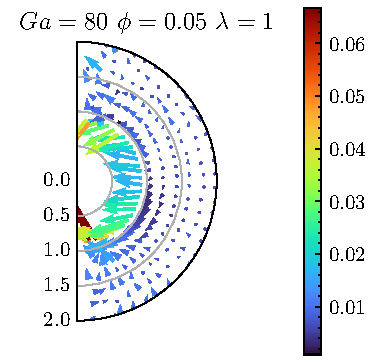
\includegraphics[width=0.3\textwidth]{image/HOMOGENEOUS_final/Dist/F_rel_l_1_Ga_80_PHI_5}
        \caption{Averaged force vector applied on the droplet present at the origin, conditioned on the presence of a nearest neighbor.
        The radial distance is made dimensionless by the droplets diameter. 
        The color map represents the magnitude of the forces.}
        \label{fig:perspective_forces}
    \end{figure}
    On \ref{fig:perspective_forces} we display our first result regarding the interaction force statistics. 
    One can remark that \ref{fig:perspective_forces} is a visual representation of the particle-fluid-particle stress (as defined in \citep{zhang2021ensemble}). 
\end{enumerate}


Then there are the projects that might be relevant to this work, 
however, at this stage, it is hard to estimate if they are all essential.
\begin{enumerate}
    \item In \ref{chap:closure-disperse} we studied the dependence of the first moment of forces on mean relative motions.
    It seems important to develop a model that is more accurate for higher Reynolds numbers and volume fractions since it could be predominant in determining the rheology of dense emulsions. 
    \item The study of the modeling of the second moment of the hydrodynamic forces seems important as well. 
    \item All the closure terms presented in this work are derived under the condition of a steady-state configuration.
    It means that we neglected the contribution from the relative phase acceleration. 
    For the drag force we know that that added mass effects cannot be neglected. 
    For the higher moments of force, this kind of contributions must be determined as well. 
    \item Likewise, we considered homogeneous rising emulsions, however, we may take into account the gradient of droplet concentration in all of our closure terms. 
    The recent study of \citet{wang2024effect} started to investigate the effect of volume fraction gradient  ($\grad\phi$) on the drag force closure for example.  
    \item 
    Obtaining closure terms using  Particule-Resolved DNS can be quite expensive. 
    % PR-DNS (Particle-Resolve Direct-Numerical-Simulations) can be quite expansive to develop closure terms. 
    Thus, one might consider solving the single-particle conditioned averaged equations to build closure terms.  
    Indeed, as demonstrated by \citet{hinch1977averaged} by considering closures within those equations one can derive more complete closure terms (such as the second-order correction of the equivalent stress and sedimentation velocity in his case). 
    Nevertheless, this approach is theoretically difficult, limiting the number of problems that can be treated. 
    Solving these equations using a numerical approach would enable us to consider more complicated scenarios. 
    For example, we could prescribe a given pair distribution function in the equations; it would represent the mean gradient of volume fraction, layers in the microstructure etc. 
    Then, it would lead to closure models in terms of that given pair distribution. 
\end{enumerate}

Overall, a significant amount of work remains to be done to model, at least, the closure terms of the averaged momentum equations. 
Indeed, the scalar functions $C_1$ and $C_2$ in \ref{eq:stress}, represent the contribution of the stresslet, Reynolds stress, and particle-fluid-particle stress tensor \citep{zhang2021ensemble}, therefore $C_1$ and $C_2$ require at least 6 closure laws (two for each contribution). 
Likewise, the effective stress of the dispersed phase may also include contact stresses and particle-fluid-particle interactions.  

I believe that to archive major advances in the modeling of buoyancy-driven dispersed multiphase flows, one must now find a way to measure directly the scalar functions $C_1$ and $C_2$, from numerical or laboratory experiments.
In other words, it would be nice to develop a tool of measurement that can directly measure $C_1$ and $C_2$, analogous to how a rheometer measures the equivalent viscosity of a mixture (i.e. $\mu_f(1+C_E)$ in \ref{eq:stress}). 
This approach may be more accurate and more simple, as 
it would circumvent the need for building independent closures for each term in the effective stresses (as done in this work). 
To address cases of non-homogeneous flows, one must consider the other scalar functions presented in \ref{ap:momentum_formulation}.  